\documentclass[a4paper,hidelinks,14pt]{extarticle}

\usepackage[utf8]{inputenc}
\usepackage[T2A]{fontenc}
\usepackage[english, russian]{babel}
\usepackage{amsmath}
\usepackage{amsfonts}
\usepackage{mathtools}
\usepackage{datetime}
\usepackage[pdftex]{graphicx}
\usepackage{indentfirst}
\usepackage{asymptote}
\usepackage{systeme}
\usepackage{listings}
\usepackage[usenames,dvipsnames]{color}	
\usepackage[font={small,it}]{caption}
\usepackage{gensymb}
\usepackage{hyperref}
\newcommand{\Span}{\text{Span}}
\newcommand{\Img}{\text{Im}}
\newcommand{\Ker}{\text{Ker}}
\hypersetup{
	colorlinks=true,
	linkcolor=blue,
	filecolor=magenta,      
	urlcolor=cyan,
}

\begin{document}
	\begin{titlepage}
		
		\setlength{\parindent}{0ex}
		
		\begin{center}
			\textsc{
				\vspace{1ex}
				Научно исследовательский университет ИТМО \\
				\vspace{0.5ex}
				Факультет систем управления и робототехники \\
				\vspace{0.5ex}
			}
		\end{center}
		
		\vspace{50mm}
		
		\begin{center}
			Отчет по лабораторной работе №2 \\
			2D-преобразования
		\end{center}
		
		\vspace{50mm}
		
		\begin{minipage}{.55\linewidth}
			Выполнил студент группы R3280
			
			\smallskip
			
			Преподаватель
		\end{minipage}
		\hfill
		\begin{minipage}{.4\linewidth}
			\begin{flushright}
				Мовчан И. Е.
				\\
				Перегудин А. А.
			\end{flushright}
		\end{minipage}
		
		\vfill
		\begin{center}
			Санкт-Петербург
			\\
			2024
		\end{center}
		
	\end{titlepage}
	
	Перед выполнением выберем различные четыре целых числа, причем такие, что ни одно из них не равнялось $0$ или $\pm1$.
	
	Итак, $a=2$, $b=3$, $c=6$, $d=9$. Теперь можем начинать делать наши преобразования матрицами $2\times2$!
	
	\section{Придумываем}
	\subsection{Отражение плоскости относительно прямой \\ $y=ax=2x$}
	Для нахождения этой матрицы воспользуемся тем фактом, что перпендикулярная прямая задаётся уравнением $y=-\frac{1}{2}x + C$. Пользуясь этим фактом и построениями в desmos, можем найти, куда должны перейти базисные вектора $(0, 1)$ и $(1, 0)$, а после составить матрицу:
	\begin{figure}[h]
		\centering
		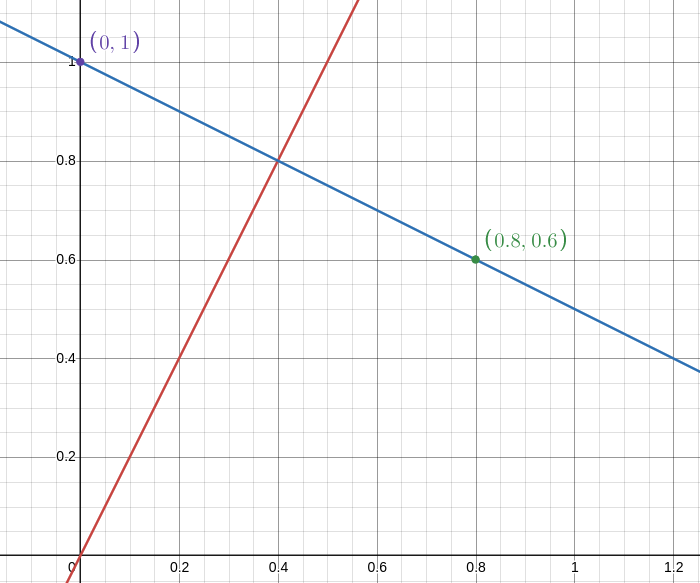
\includegraphics[width=10cm, height=8cm]{1.png}
		\caption{Пример вычисления для $(0,1)$}
	\end{figure}
	
	Матрица тогда будет выглядеть следующим образом:
	$$
	A = \begin{bmatrix}
		-0.6 & 0.8 \\
		\phantom{-}0.8 & 0.6
	\end{bmatrix}
	$$
	\subsection{Отражение плоскости в прямую $y=bx=3x$}
	Аналогично пункту выше найдём, куда переходят <<базисные точки>> через решение систем на пересечение прямой и ей перпендикулярной, проходящей через точки $(0,1)$ и $(1,0)$, либо, если решение получаются простыми, через desmos. У нас последний случай, поэтому можем сразу дать ответ:
	$$
	A = \begin{bmatrix}
		0.1 & 0.3 \\
		0.3 & 0.9
	\end{bmatrix}
	$$
	Сопроводим это примером:
	\begin{figure}[h]
		\centering
		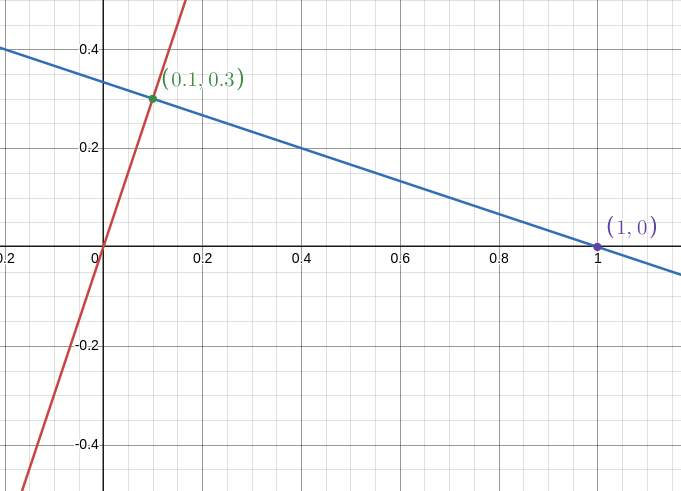
\includegraphics[width=10cm, height=8cm]{2.png}
		\caption{Пример вычисления для $(1,0)$}
	\end{figure}
	\subsection{Поворот плоскости на $10c=60\degree=\frac{\pi}{3}$}
	Поворот будет осуществлятьс яв положительном направлении, то есть против часовой стрелки.
	
	Тут совсем всё просто, ведь мы знаем нашу матрицу поворота, нужно лишь подставить значения, получив:
	$$
	A = \begin{bmatrix}
		\cos(\frac{\pi}{3}) & -\sin(\frac{\pi}{3}) \\
		\sin(\frac{\pi}{3}) & \phantom{-}\cos(\frac{\pi}{3})
	\end{bmatrix}
	=\begin{bmatrix}
		\frac{1}{2} & -\frac{\sqrt{3}}{2} \\
		\frac{\sqrt{3}}{2} & \phantom{-}\frac{1}{2}
	\end{bmatrix}
	$$
	\subsection{Центральная симметрия плоскости}
	Осуществляется относительно начала координат, а значит, ситуация очень простая - нужно лишь поменять знаки у $x$ и $y$ (если мы рассматриваем точку $(x, y)$). Матрица получается следующей:
	$$
	A = \begin{bmatrix}
		-1 & \phantom{-}0 \\
		\phantom{-}0 & -1
	\end{bmatrix}
	$$
	\subsection{Композиция отображений}
	Отображение описывается так:  сначала отражение относительно прямой $y = ax = 2x$, потом поворот на $10d=90\degree=\frac{\pi}{2}$ по часовой стрелке. Вышеописанное является композицией отображений, матрицы которых мы уже знаем, а значит, чтобы получить требуемое, нужно лишь их перемножить:
	$$
	A = A_1 A_2 = \begin{bmatrix}
		-0.6 & 0.8 \\
		\phantom{-}0.8 & 0.6
	\end{bmatrix}
	\begin{bmatrix}
		\cos(\frac{\pi}{2}) & -\sin(\frac{\pi}{2}) \\
		\sin(\frac{\pi}{2}) & \phantom{-}\cos(\frac{\pi}{2})
	\end{bmatrix}
	=	
	\begin{bmatrix}
		0.8 & \phantom{-}0.6 \\
		0.6 & -0.8
	\end{bmatrix}
	$$
	\subsection{Отображение смены базиса}
	Отображение должно переводить прямую $y = 0$ в $y=ax=2x$ и $x=0$ в $y=bx=3x$. Матрица задаётся через действие на базис:
	$$
	\begin{bmatrix}
		f & g \\
		h & k
	\end{bmatrix}
	\begin{bmatrix}
		1 \\
		0
	\end{bmatrix}
	=
	\begin{bmatrix}
		f \\
		h
	\end{bmatrix}
	=
	\begin{bmatrix}
		1 \\
		2a
	\end{bmatrix}
	=
	\begin{bmatrix}
		1 \\
		2
	\end{bmatrix}
	$$
	$$
	\begin{bmatrix}
		f & g \\
		h & k
	\end{bmatrix}
	\begin{bmatrix}
		0 \\
		1
	\end{bmatrix}
	=
	\begin{bmatrix}
		g \\
		k
	\end{bmatrix}
	=
	\begin{bmatrix}
		1 \\
		3b
	\end{bmatrix}
	=
	\begin{bmatrix}
		1 \\
		3
	\end{bmatrix}
	$$
	Итого, получаем следующую матрицу отображения:
	$$
	A = \begin{bmatrix}
		1 & 1 \\
		2 & 3
	\end{bmatrix}
	$$
	
	\subsection{Обратное отображение}
	Хотим сделать обратное преобразование от предыдущего пункта: перейти из прямой $y=ax=2x$ в прямую $y=0$, а из $y=bx=3x$ в $x=0$. Но ведь это делается элементарным взятием обратного:
	$$
	A = 
	\begin{bmatrix}
		1 & 1 \\
		2 & 3
	\end{bmatrix}^{-1}
	=
	\begin{bmatrix}
		\phantom{-}3 & -1 \\
		-2 & \phantom{-}1
	\end{bmatrix}
	$$
	\subsection{Перемена мест прямых}
	Теперь нам необходимо отображение, меняющее местами $y=ax=2x$ и $y=bx=3x$.
	
	Найдём прямую, точки которой равноудалены от наших прямых, а после сделаем симметричное отображение. Искомая прямая задаётся уравнением $y=kx=\tg(\frac{\arcctg(2)+\arcctg(3)}{2})x=\tg(\frac{3\pi}{8})x$. Для поиска матрицы отображения необходимо решить следующие уравнения:
	$$\tg(\frac{3\pi}{8})x = -\frac{1}{\tg(\frac{3\pi}{8})}x+1$$
	
	Откуда получаем $x=\frac{1}{2\sqrt{2}}$, симметричная точка тогда будет иметь координаты $x=\frac{1}{\sqrt{2}}, y=-\frac{1}{\tg(\frac{3\pi}{8})\sqrt{2}}+1=\frac{1}{\sqrt{2}}$
	
	По аналогичным соображениям можем из уравнения $$\tg(\frac{3\pi}{8})x = -\frac{1}{\tg(\frac{3\pi}{8})}x+\frac{1}{\tg(\frac{3\pi}{8})}$$
	
	Получить симметричную точку с координатами $x=-\frac{1}{\sqrt{2}}, y = \frac{1}{\sqrt{2}}$.
	
	В итоге имеем:
	$$
	A = 
	\begin{bmatrix}
		-\frac{1}{\sqrt{2}} & \frac{1}{\sqrt{2}} \\
		\phantom{-}\frac{1}{\sqrt{2}} & \frac{1}{\sqrt{2}}
	\end{bmatrix}
	$$
	
	\pagebreak
	Небольшая иллюстрация к произошедшему:
	\begin{figure}[h]
		\centering
		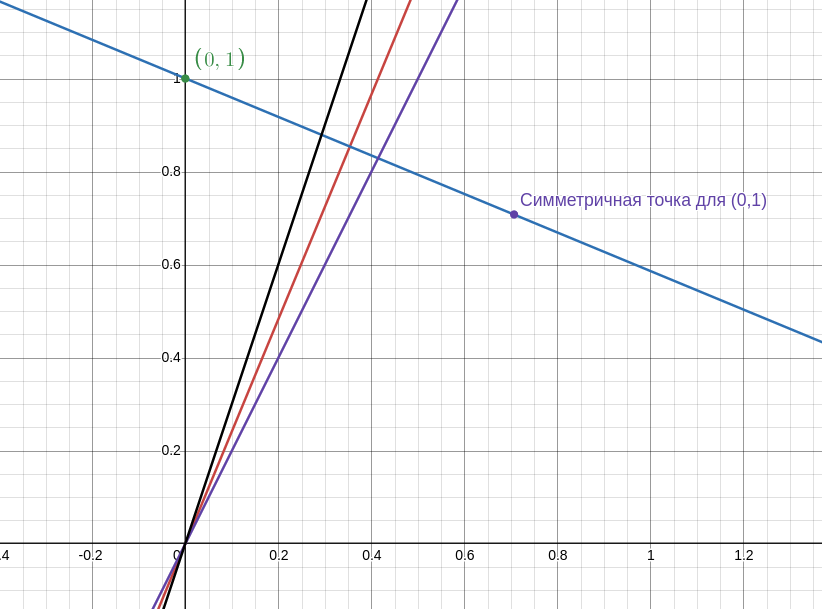
\includegraphics[width=10cm, height=8cm]{3.png}
		\caption{Пример вычисления для $(0,1)$}
	\end{figure}
	
	\subsection{Увеличение площади единичного круга}
	Хотим увеличить площадь единичного круга с началом в центре координат до $c=6$. Данное делает отображение, задающееся следующей матрицей:
	$$
	A = \begin{bmatrix}
		\sqrt{6} & 0 \\
		0 & \sqrt{6}
	\end{bmatrix}
	$$
	
	\subsection{Превращение в не круг}
	Необходимо, как и в прошлом пункте, увеличить площадь круга до $d=9$, при этом испортить его, сделав круг не кругом. Данное возможно с помощью следующей матрицы:
	$$
	A = \begin{bmatrix}
		1 & 0 \\
		0 & 9
	\end{bmatrix}
	$$
	
	Круг при данном отображении превратится в эллипс.
	
	\subsection{Отображение с перпендикулярными собственными векторами, не лежащими на $y=0$ и $y=x$}
	Восстановим матрицу через спектральное разложение, взяв за собственные вектора $v_1=\begin{bsmallmatrix}
		1 \\
		2
	\end{bsmallmatrix}
	$ и $v_2=\begin{bsmallmatrix}
		-2 \\
		1
	\end{bsmallmatrix}
	$ (они перпендикулярны, так как их скалярное произведение равно 0), а за собственные числа $\lambda_1=1, \lambda_2=2$:
	$$
	A =
	\begin{bmatrix}
		1 & -2 \\
		2 & \phantom{-}1
	\end{bmatrix}
	\begin{bmatrix}
		1 & 0 \\
		0 & 2
	\end{bmatrix}
	\begin{bmatrix}
		1 & -2 \\
		2 & \phantom{-}1
	\end{bmatrix}^{-1}
	=
	\begin{bmatrix}
		\phantom{-}1.8 & -0.4 \\
		-0.4 & \phantom{-}1.2
	\end{bmatrix}
	$$
	\subsection{Отображение без двух коллинеарных собственных векторов}
	Нужно лишь взять матрицу, определитель которой равен 0 (отметим также, что это по сути является отображением в прямую):
	$$
	A = \begin{bmatrix}
		2 & 3 \\
		4 & 6
	\end{bmatrix}
	$$
	\subsection{Отображение с комплексными векторами}
	Необходимо придумать матрицу, у которой нет ни одного вещественного собственного вектора, но сама она при этом будет вещественной.
	Данному условию удовлетворяет матрица
	$$
	A = \begin{bmatrix}
		0 & -1 \\
		1 & 0
	\end{bmatrix}
	$$
	
	Уравнение на собственные числа не будет решаться в вещественном случае, т.к. получаем $\lambda^{2}=-1$, а значит, и собственные вектора матрицы будут комплексными.
	
	\subsection{Отображение, для которого любой ненулевой вектор является собственным}
	Данному условию удовлетворяет матрицы расширения/сужения пространства, одной из таких является следующая:
	$$
	A = \begin{bmatrix}
		5 & 0 \\
		0 & 5
	\end{bmatrix}
	$$
	\subsection{Некоммутативные отображения}
	Необходимо придумать некоммутативные матрицы $A$ и $B$.
	
	Пусть
	$$A = \begin{bmatrix}
		0 & \phantom{-}1 \\
		2 & -1
	\end{bmatrix}, \text{ } B = \begin{bmatrix}
	-1 & 0 \\
	\phantom{-}1 & 2
	\end{bmatrix}$$.
	
	Тогда
	
	$$
	AB = \begin{bmatrix}
		\phantom{-}1 & \phantom{-}2 \\
		-3 & -2
	\end{bmatrix}
	\neq
	\begin{bmatrix}
		0 & -1 \\
		4 & -1
	\end{bmatrix} = BA
	$$
	\subsection{Коммутативные отображения}
	Всё аналогично предыдущему пункту (матрицы ищем из соображений о том, что собственные вектора должны быть одинаковыми):
	$$
	A = \begin{bmatrix}
		2 & 1 \\
		3 & 4
	\end{bmatrix}, \text{ }
	B = \begin{bmatrix}
		3 & 1 \\
		3 & 5
	\end{bmatrix}
	$$
	
	$$
	AB = BA = \begin{bmatrix}
		9 & 7 \\
		21 & 23
	\end{bmatrix}
	$$
	
	\section{Анализируем}
	\subsection{Образ и ядро}
	Для \textit{1} пункта: $$\Img(A) = \Span\{\begin{bmatrix}
		-0.6 \\ 0.8
	\end{bmatrix}, \begin{bmatrix}
		0.8 \\ 0.6
	\end{bmatrix}\}, \Ker(A)=\{\begin{bmatrix}
	0 \\ 0
	\end{bmatrix}\}$$
	
	Для \textit{2} пункта: $$\Img(A) = \Span\{\begin{bmatrix}
		0.1 \\ 0.3
	\end{bmatrix}\}, \Ker(A)=\Span\{\begin{bmatrix}
		-3 \\ 1
	\end{bmatrix}\}$$
	
	Для \textit{13} пункта: 
	$$\Img(A) = \Span\{\begin{bmatrix}
		0 \\ 1
	\end{bmatrix}, \begin{bmatrix}
		1 \\ 0
	\end{bmatrix}\}, \Ker(A)=\{\begin{bmatrix}
		0 \\ 0
	\end{bmatrix}\}$$
	
	Для \textit{14} пункта: 
	$$\Img(A) = \Span\{\begin{bmatrix}
		5 \\ 0
	\end{bmatrix}, \begin{bmatrix}
		0 \\ 5
	\end{bmatrix}\}, \Ker(A)=\{\begin{bmatrix}
		0 \\ 0
	\end{bmatrix}\}$$
	
	\subsection{Собственные числа и вектора}
	Для \textit{1} пункта:
	$$
	v_1=\begin{bmatrix}
		1 \\ 2
	\end{bmatrix}, \text{ }
	v_2 = \begin{bmatrix}
		-2 \\ 1
	\end{bmatrix}, \text{ }
	\lambda_1 = 1, \text{ }
	\lambda_2 = -1
	$$
	
	Для \textit{2} пункта:
	$$
	v_1=\begin{bmatrix}
		-3 \\ 1
	\end{bmatrix}, \text{ }
	v_2 = \begin{bmatrix}
		1 \\ 3
	\end{bmatrix}, \text{ }
	\lambda_1 = 0, \text{ }
	\lambda_2 = 1
	$$
	
	Для \textit{3} пункта:
	$$
	v_1=\begin{bmatrix}
		-i \\ 1
	\end{bmatrix}, \text{ }
	v_2 = \begin{bmatrix}
		i \\ 1
	\end{bmatrix}, \text{ }
	\lambda_1 = \frac{1-i\sqrt{3}}{2}, \text{ }
	\lambda_2 = \frac{1+i\sqrt{3}}{2}
	$$
	
	Для \textit{4} пункта:
	$$
	v_1=\begin{bmatrix}
		1 \\ 0
	\end{bmatrix}, \text{ }
	v_2 = \begin{bmatrix}
		0 \\ 1
	\end{bmatrix}, \text{ }
	\lambda_1 = -1, \text{ }
	\lambda_2 = -1
	$$
	
	Для \textit{8} пункта:
	$$
	v_1=\begin{bmatrix}
		\sqrt{2} - 1 \\ 1
	\end{bmatrix}, \text{ }
	v_2 = \begin{bmatrix}
		-\sqrt{2} - 1 \\ 1
	\end{bmatrix}, \text{ }
	\lambda_1 = 1, \text{ }
	\lambda_2 = -1
	$$
	
	Для \textit{11} пункта:
	$$
	v_1=\begin{bmatrix}
		-1 \\ 2
	\end{bmatrix}, \text{ }
	v_2 = \begin{bmatrix}
		-2 \\ 1
	\end{bmatrix}, \text{ }
	\lambda_1 = 1, \text{ }
	\lambda_2 = 2
	$$
	
	Для \textit{12} пункта:
	$$
	v_1=\begin{bmatrix}
		-3 \\ 2
	\end{bmatrix}, \text{ }
	v_2 = \begin{bmatrix}
		1 \\ 2
	\end{bmatrix}, \text{ }
	\lambda_1 = 0, \text{ }
	\lambda_2 = 8
	$$
	
	Для \textit{13} пункта:
	$$
	v_1=\begin{bmatrix}
		i \\ 1
	\end{bmatrix}, \text{ }
	v_2 = \begin{bmatrix}
		-i \\ 1
	\end{bmatrix}, \text{ }
	\lambda_1 = i, \text{ }
	\lambda_2 = -i
	$$
	
	Для \textit{14} пункта:
	$$
	v_1=\begin{bmatrix}
		1 \\ 0
	\end{bmatrix}, \text{ }
	v_2 = \begin{bmatrix}
		0 \\ 1
	\end{bmatrix}, \text{ }
	\lambda_1 = 5, \text{ }
	\lambda_2 = 5
	$$
	
	Для \textit{15} пункта:
	$$
	v_{1A}=\begin{bmatrix}
		-1 \\ 2
	\end{bmatrix}, \text{ }
	v_{2A} = \begin{bmatrix}
		1 \\ 1
	\end{bmatrix}, \text{ }
	\lambda_{1A} = -2, \text{ }
	\lambda_{2A} = 1
	$$
	$$
	v_{1B}=\begin{bmatrix}
		-3 \\ 1
	\end{bmatrix}, \text{ }
	v_{2B} = \begin{bmatrix}
		0 \\ 1
	\end{bmatrix}, \text{ }
	\lambda_{1B} = -1, \text{ }
	\lambda_{2B} = 2
	$$
	
	Для \textit{16} пункта:
	$$
	v_{1A}=\begin{bmatrix}
		-1 \\ 1
	\end{bmatrix}, \text{ }
	v_{2A} = \begin{bmatrix}
		1 \\ 3
	\end{bmatrix}, \text{ }
	\lambda_{1A} = 1, \text{ }
	\lambda_{2A} = 5
	$$
	$$
	v_{1B}=\begin{bmatrix}
		-1 \\ 1
	\end{bmatrix}, \text{ }
	v_{2B} = \begin{bmatrix}
		1 \\ 3
	\end{bmatrix}, \text{ }
	\lambda_{1B} = 2, \text{ }
	\lambda_{2B} = 6
	$$
	\subsection{Определители}
	Для \textit{1} пункта: $\det(A) = -1$
	
	\vspace{1mm}
	
	Для \textit{2} пункта: $\det(A) = 0$
	
	\vspace{1mm}
	
	Для \textit{3} пункта: $\det(A) = 1$
	
	\vspace{1mm}
	
	Для \textit{4} пункта: $\det(A) = 1$
	
	\vspace{1mm}
	
	Для \textit{5} пункта: $\det(A) = -1$
	
	\vspace{1mm}
	
	Для \textit{6} пункта: $\det(A) = 6$
	
	\vspace{1mm}
	
	Для \textit{9} пункта: $\det(A) = 9$
	
	В 5 и 9 пунктах получили зависимость детерминанта от увеличения площади. Площадь увеличилась в количество раз, равному значению определителя!
	
	\subsection{Обязательная симметричность}
	Матрицы должны быть обязательно симметричными для пунктов 1, 4, 5 - не зря ведь эти преобразования симметричные, 11 и 14.
	
	\section{Визуализируем}
	Будем делать визуализацию с помощью manim. Вот \href{https://drive.google.com/drive/folders/1UD4GCDIHPwfSrOiIkLXwKyiMfg2L4nb8?usp=sharing}{ссылка} на диск со всеми анимациями. Отметим, что в анимациях после применения матриц собственные вектора отображений уже будут показаны и учтены, так что не имеет смысла добавлять их дополнительно.
	
	\textbf{На этом всё, спасибо!}
\end{document}